\documentclass{article}
\usepackage{graphicx}
\usepackage{imakeidx}


\title{Git for Robots}   
\author{Arjun Gandhi} 
\date{\today} 

\begin{document}


%=========================================
\begin{titlepage}
		\centering{
			{\fontsize{40}{48}\selectfont 
			Git for Robotics}
		}\\
			
		\vspace{10mm}
		\centering{\Large{Arjun Gandhi}}\\
		\vspace{\fill}
		\centering \large{March 2020}
\end{titlepage}


%=========================================
\newpage{}
\thispagestyle {empty}

\vspace*{2cm}

\begin{figure}
		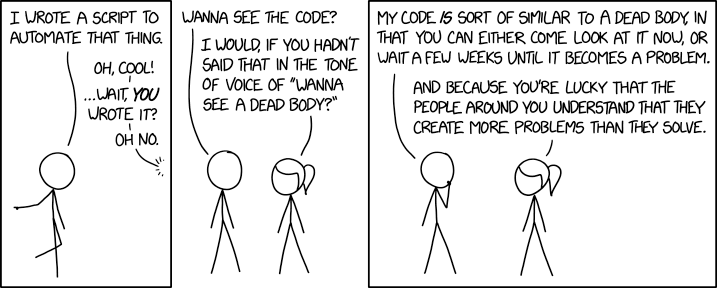
\includegraphics[width=5.5in]{images/wanna_see_the_code.png}
		\caption{This is how all of my robotics project go.}
\end{figure}

\newpage

\tableofcontents

\newpage
\section{What is version control?}
\paragraph{}
    You can think of a version control system (short: "VCS\index{VCS}") as a kind of "database". It lets you save a snapshot of your complete project at any time you want. When you later take a look at an older snapshot (let's start calling it "version\index{version}"), your VCS shows you exactly how it differed from the previous one.
    \includegraphics[5.5in]{}
    
    
    Version control is independent of the kind of project / technology / framework you're working with:
    \begin{itemize}
        \item It works a website as it does for a robotics project
        \item It lets you work with any tool you like; it doesn't care what kind of text editor, graphics program, file manager or other tool you use
    \end{itemize}

    At the core of it a VCS records the changes you make to your project's files. This is what version control is about. It's really as simple as it sounds.
\subsection{Why use version control}

\subsection{Types of version control}
\subsection{Why use git?}
\section{What is git and how does it work?}
\newpage{}
\thispagestyle {empty}

\vspace*{2cm}

\begin{figure}
		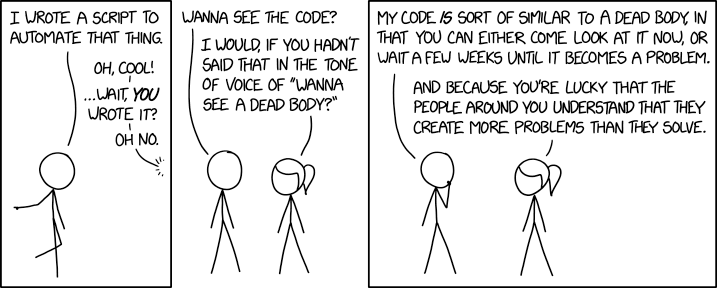
\includegraphics[width=5.5in]{images/wanna_see_the_code.png}
		\caption{This is how all of my robotics project go.}
\end{figure}

\section{How to install git}
\subsection{Command Line}
\subsection{Github Desktop App}
\subsection{Eclipse}
\subsection{Other Apps}

\section{How to use git}
\subsection{Best Practices}


\printindex

%Referances
%https://www.git-tower.com/learn/git/ebook/en/command-line/basics/why-use-version-control

\end{document}
